%%%%%%%%%%%%%%%%%%%%%%%%%%%%%%%%%%%%%%%%%%%%%%%%%%%%%%%%
% Este é um documento que servirá de modelo para
% os relatórios feitos na disciplina Circuitos Digitais
% 2016-2
%%%%%%%%%%%%%%%%%%%%%%%%%%%%%%%%%%%%%%%%%%%%%%%%%%%%%%%%%

\documentclass[12pt]{article}

\usepackage{sbc-template}
\usepackage[brazil,american]{babel}
\usepackage[utf8]{inputenc}

\usepackage{graphicx}
\usepackage{url}
\usepackage{float}
\usepackage{listings}
\usepackage{color}
\usepackage{todonotes}
\usepackage{algorithmic}
\usepackage{algorithm}
\usepackage{hyperref}
\usepackage{indentfirst}

\sloppy

\title{Projeto Final\\ 
	Dados abertos do Bolsa Família}

\author{Dayanne Fernandes da Cunha, 13/0107191\\
	 Christian Costa Werner ,  14/0134573
}

\address{Dep. Ciência da Computação -- Universidade de Brasília (UnB)\\
	Banco de Dados - Turma A
	\email{dayannefernandesc@gmail.com, ccwerner96@gmail.com}
}

\begin{document} 
	\maketitle
	
	\selectlanguage{american}
	\begin{abstract}
		This report corresponds to the step-by-step project of creating a database using open data from the federal government (transparency portal). We will answer some issues about \textit{Bolsa Familia} theme.
	\end{abstract}
	\selectlanguage{brazil}     
	
	\begin{resumo} 
		Este relatório corresponde ao passo a passo do projeto de criação de um banco de dados utilizando dados públicos do governo federal (portal da transparência). Iremos sanar algumas questões sobre o tema \textit{Bolsa Família}.
	\end{resumo}
	
	\tableofcontents
	\newpage 
	
	\section{Introdução}
	\label{sec:intro}
	
	\subsection{Motivação}
	\label{sec:motiv}
	
	Este relatório se deve ao Projeto de Banco de Dados da disciplina de Banco de Dados da Universidade de Brasília (UnB), referente ao segundo semestre de 2016, turma A. Esse projeto consiste em montar um Banco de Dados com os dados do governo do programa Bolsa Família - setembro de 2015, segundo disponível no \cite{portal}.
	
	Este relatório abrange o que é o programa social Bolsa Família e todo um passo-a-passo de criação de um banco de dados, partindo de um arquivo maciço CSV \emph{(Comma-Separated Values)} usando as mais variadas ferramentas (para verificar as ferramentas, visite o item \ref{sec:proj} e confira o \emph{README} do projeto).
	
	\subsection{Programa Social - Bolsa Família}
	\label{sec:psbf}
	
	\subsubsection{Sobre o Programa}
	\label{sec:bfsobre}
	
	O Programa Bolsa Família - PBF é um programa de transferência de renda do Governo Federal, sob condicionalidades, instituído no Governo Lula pela Medida Provisória 132, de 20 de outubro de 2003, convertida em lei em 9 de janeiro de 2004, pela Lei Federal n. 10.836.
	
	Tendo sido apelidado de \emph{Programa 1335 – Transferência de Renda com Condicionalidades – Bolsa Família}, foram geradas ações de controle com o fito de avaliar a efetiva aplicação dos recursos destinados ao cumprimento da finalidade constante da \emph{Ação 8442 – Transferência de Renda Diretamente às Famílias em Condições de Pobreza e Extrema Pobreza}, pertencente ao \emph{Programa Bolsa Família - PBF}.
	
	O objetivo do programa \emph{1335 – Transferência de Renda com Condicionalidades – Bolsa Família} é Combater a fome, a pobreza e outras formas de privação das famílias e promover a segurança alimentar e nutricional e o acesso à rede de serviços públicos de saúde, educação e assistência social, criando possibilidades de emancipação sustentada dos grupos familiares e de desenvolvimento local dos territórios.
	
	O objetivo da ação \emph{8442 – Transferência de Renda Diretamente às Famílias em Condições de Pobreza e Extrema Pobreza} é Melhorar as condições socioeconômicas das famílias pobres e extremamente pobres por meio de transferência direta de renda.
	
	A gestão do PBF é descentralizada e compartilhada por União, estados, Distrito Federal e municípios. Estes entes federados trabalham em conjunto para aperfeiçoar, ampliar e fiscalizar a execução do Programa, instituído pela Lei 10.836/04 e regulamentado pelo Decreto nº 5.209/04.
	
	As famílias beneficiárias são selecionadas com base nas informações inseridas pelo município no Cadastro Único para Programas Sociais (Cadastro Único). O Cadastro é um instrumento de coleta de dados que tem como objetivo identificar todas as famílias de baixa renda existentes no País. A seleção dos beneficiários é realizada de forma automatizada, utilizando-se como principal critério a renda per capita da família.
	
	Os Órgãos Federais envolvidos na execução do Programa são: a SECRETARIA NACIONAL DE RENDA DE CIDADANIA DO MINISTÉRIO DO DESENVOLVIMENTO SOCIAL E COMBATE À FOME - SENARC/MDS (UG: 550007), responsável pela coordenação, gestão e operacionalização do Programa Bolsa Família; a CAIXA ECONÔMICA FEDERAL (CAIXA), com a função de Agente Operador do PBF, mediante remuneração e condições pactuadas no contrato com o MDS; o MINISTÉRIO DA SAÚDE – MS, por meio da Secretaria de Atenção a Saúde (UG 250010), responsável pela gestão federal do acompanhamento do cumprimento das condicionalidades de saúde das famílias beneficiárias do PBF; o MINISTÉRIO DA EDUCAÇÃO - MEC, por meio da Secretaria de Educação Continuada, Alfabetização e Diversidade (UG: 150028), responsável pela gestão federal do sistema de frequência escolar dos alunos; e a SECRETARIA NACIONAL DE ASSISTÊNCIA SOCIAL DO MINISTÉRIO DO DESENVOLVIMENTO SOCIAL E COMBATE À FOME – SNAS/MDS (UG 550011), responsável em realizar a coleta e o registro periódico das informações referentes à condicionalidade da assistência social.
	
	Os demais órgãos responsáveis, governos estaduais com a função de apoiar os municípios na implementação do Programa; governos municipais e Distrito Federal, responsáveis pela gestão local do Programa Bolsa Família e do Cadastro Único; e Órgãos de Controle Social, responsáveis por garantir aos cidadãos espaço para o acompanhamento do Programa, atuam visando assegurar os interesses da sociedade, bem como permitir que suas demandas e necessidades sejam apresentadas ao poder público.
	
	\subsubsection{Volume de recursos envolvidos}
	\label{sec:vre}
	
	Os volumes de recursos orçamentários destinados à Ação 8442 - Transferência de Renda Diretamente às Famílias em Condição de Pobreza e Extrema Pobreza (Lei nº 10.836/2004) para os exercícios entre 2007 a 2012 estão a seguir representados:
	
	\begin{figure}[H]
		\centering
		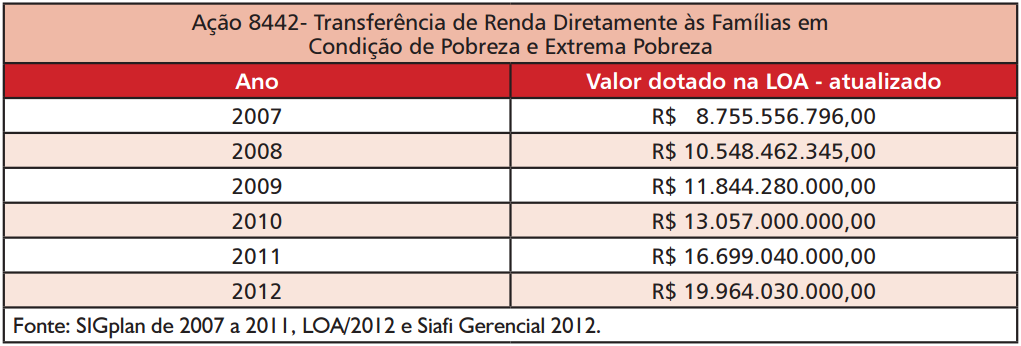
\includegraphics[width=1\textwidth]{vre_07-12.png}
		\caption{Quantidade de recursos envolvidos investido no PBF nos anos de 2007 a 2012.}
		\label{fig:vre_07-12}
	\end{figure}
	
	Podemos ver também, com dados mais atualizados, a correção monetária sobre os investimentos do PBF, e que, embora crescente, vem tendo um ritmo desacelerado, devido à crise financeira que vem assolando o Brasil nos últimos tempos. Segue então um infográfico simples que revela o investimento no PBF e as variações nominal e real nos anos de 2010 a 2016:
	
	\begin{figure}[H]
		\centering
		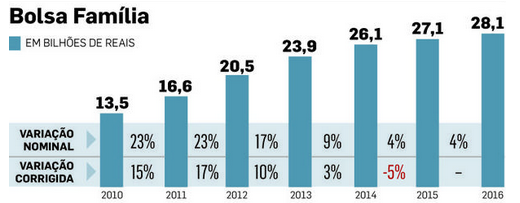
\includegraphics[width=1\textwidth]{inf_10_16.png}
		\caption{Infográfico representando o investimento em bilhões de reais e as variações nominal e corrigida sobre o PBF nos anos de 2010 a 2016.}
		\label{fig:inf_10_16}
	\end{figure}
	
	Os dados referentes à setembro de 2015 serão abordados posteriormente junto ao desenvolvimento do banco.
	
	\subsection{O Projeto}
	\label{sec:proj}
	
	Este projeto foi desenvolvido com o fim de poder analisar os dados abertos do Programa Bolsa Família – PBF. Todos os algoritmos, scripts e imagens comentadas neste relatório podem ser encontrados no repositório aberto do GitHub criado para o desenvolvimento deste projeto: \url{https://github.com/Dayof/OpenData_BolsaFamilia}. 
	
	\section{Diagrama de Entidade Relacionamento (DER)}
	\label{sec:der}
	
	O Diagrama de Entidade Relacionamento do sistema, apresentado na Figura~\ref{fig:der} foi feito pensando já no MR, e depois alterado conforme a normalização no MR foi sendo realizada. A ferramenta utilizada para desenhar o diagrama foi a \cite{lucid}. Temos no DER 7 entidades, das quais duas são entidades fracas. 
	
	\begin{figure}[H]
		\centering
		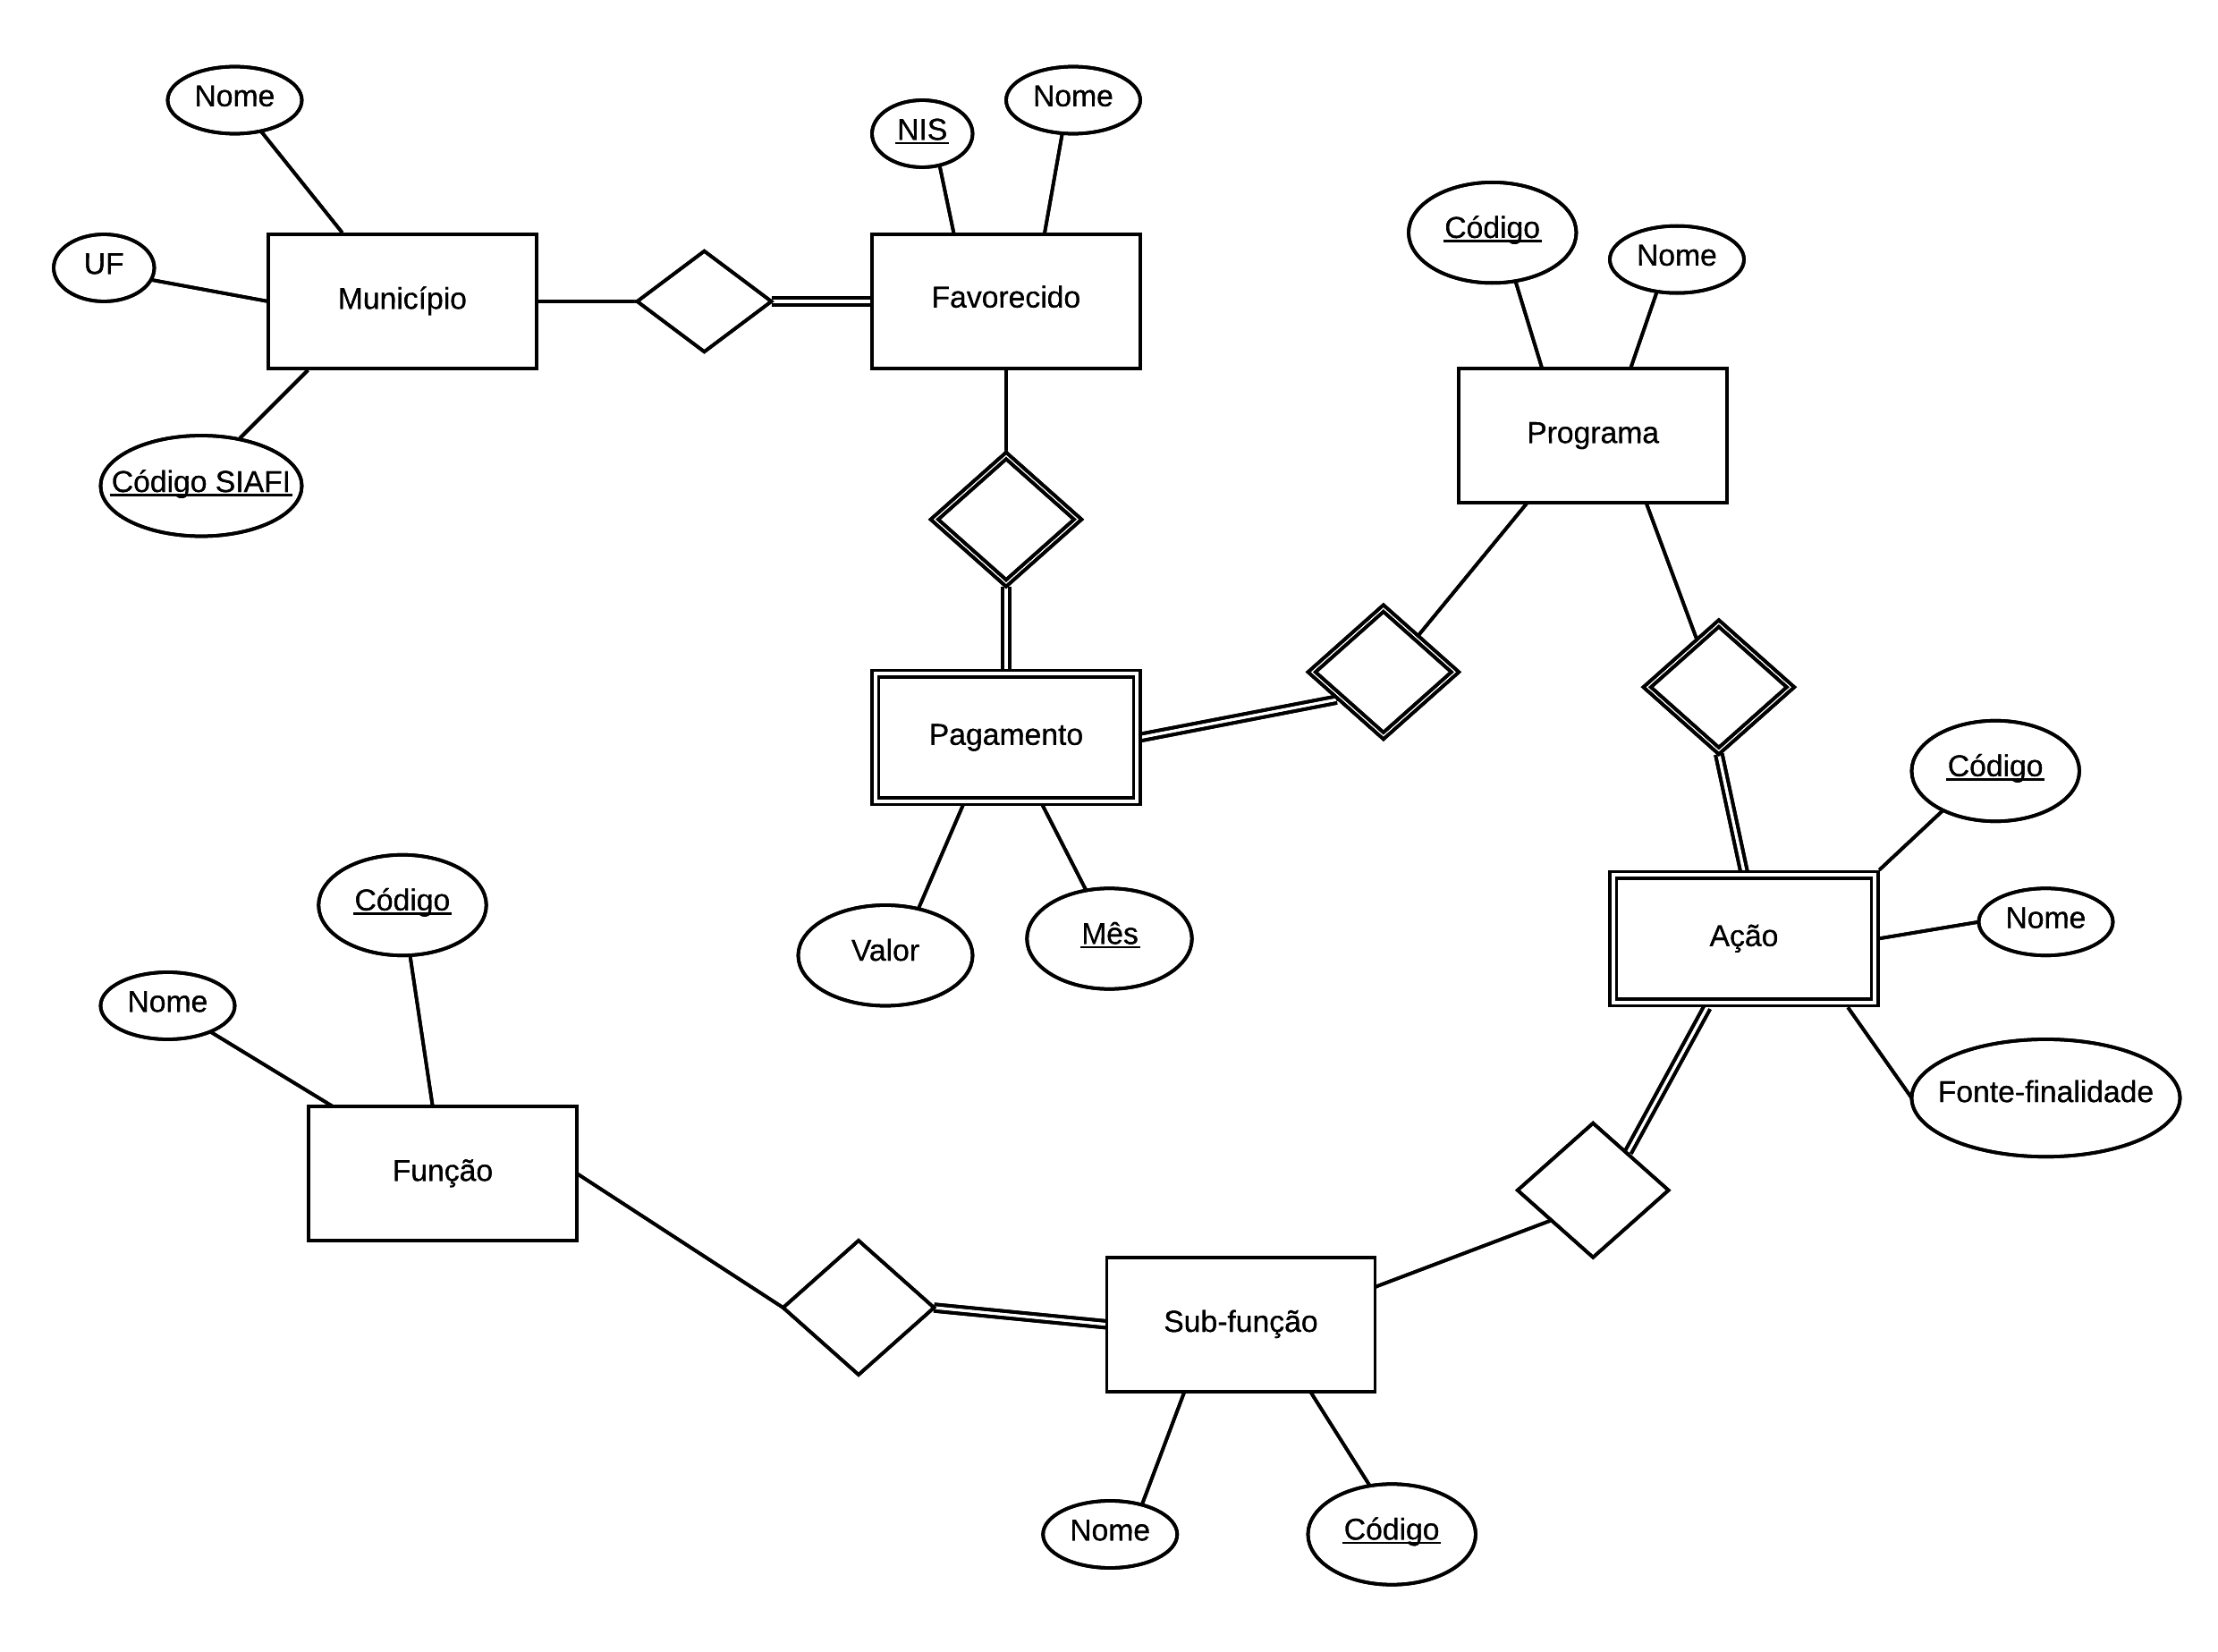
\includegraphics[width=1\textwidth]{der.png}
		\caption{Diagrama de entidade relacionamento do banco de dados dos pagamentos do Programa Bolsa Família (PBF).}
		\label{fig:der}
	\end{figure}
	
	A entidade \textbf{PAGAMENTO} é na verdade uma relação de multiplicidade N:N entre as entidades \textbf{FAVORECIDO} e \textbf{PROGRAMA}, porém, devido o programa utilizado para desenhar o DER, o \cite{lucid} apresentar problemas para inserir as multiplicidades então foi criado outra entidade para representar esta relação.
	
	\subsection{Características dos atributos do DER}
	\label{sec:atr}
	
	\begin{itemize}
		\item \textbf{UF} [MUNICIPIO] \\ Siglas dos estados. Valores repetem na tabela original do Bolsa Família.
		\item \textbf{Nome} [MUNICIPIO] \\ Nome de cada município de origem dos favorecidos, são relacionados ao Código SIAFI do município. Valores repetem na tabela original do Bolsa Família.
		\item \textbf{Código SIAFI} [MUNICIPIO] \\  É o Sistema Integrado de Administração Financeira do Governo Federal que consiste no principal instrumento utilizado para registro, acompanhamento e controle da execução orçamentária, financeira e patrimonial do Governo Federal. Valor é único para cada nome de município distinto. Valores repetem na tabela original do Bolsa Família.
		\item \textbf{Nome} [FAVORECIDO] \\ Nome de cada favorecido que recebeu pagamento do programa do bolsa família no ano de 2015 e mês de Setembro. Às vezes as folhas de pagamento contém retroativos de pagamento para algum favorecido, portanto, os valores de nome dos favorecidos repetem na tabela original do Bolsa Família.
		\item \textbf{NIS} [FAVORECIDO] \\ É uma solução que permite a identificação do trabalhador nos diversos cadastros, bem como do cidadão brasileiro beneficiário de Programas Sociais e/ou que se enquadre nas condições estabelecidas pelas Políticas Públicas de Governo Federal, Estadual ou Municipal. O NIS - Número de Identificação Social é um número de cadastro e devem ser cadastrados: o trabalhador, vinculado à empresa privada, cooperativa ou empregador pessoa física; os beneficiários de Programas Sociais (cadastrados pelo agente definido pelo Gestor do Programa); o diretor não-empregado quando optante pelo FGTS e os beneficiários de Políticas Públicas (cadastrados pela SRTE, MS e MEC). Como foi citado acima as folhas de pagamento contém retroativos de pagamento para algum favorecido, portanto, os valores de NIS dos favorecidos também repetem na tabela original do Bolsa Família.
		\item \textbf{Código} [PROGRAMA] \\  O código do programa bolsa família. Além disso, as famílias que atendem aos critérios do Programa Bolsa Família e estão inscritas em outros programas federais também têm direito ao benefício (\cite{caixa}). Os valores do código de programa podem variar em outras planilhas, porém, como está em estudo somente o programa do bolsa família o valor do código é único.
		\item \textbf{Nome} [PROGRAMA] \\ Nome oficial do programa do bolsa família oferecido pelo Governo Federal.
		\item \textbf{Código} [ACAO] \\ Código da ação do bolsa família. Análogo ao código de programa. 
		\item \textbf{Nome} [ACAO] \\ Nome oficial da ação do bolsa família oferecido pelo Governo Federal.
		\item \textbf{Fonte-Finalidade} [ACAO] \\ Possui valor igual para todos os dados da planilha coletada do portal da transparência.
		\item \textbf{Nome} [SUBFUNCAO] \\ Nome da classificação sub-funcional da despesa, exemplo: Ação Legislativa, Controle externo, etc.
		\item \textbf{Código} [SUBFUNCAO] \\ Código da classificação sub-funcional da despesa.
		\item \textbf{Nome} [FUNCAO] \\ Nome da classificação funcional da despesa, exemplo: Legislativa, Judiciária, etc.
		\item \textbf{Código} [FUNCAO] \\ Código da classificação funcional da despesa.
	\end{itemize}
	
	\subsection{Entidades do DER}
	\label{sec:ent}
	
	\begin{itemize}
		\item \textbf{MUNICIPIO} \\ Temos que a entidade \textbf{MUNICIPIO} possui 3 atributos: Nome, Código SIAFI (PK) e UF. Decidimos colocar UF como atributo pois não haveria utilidade de uma entidade para UF em si. O Código SIAFI foi escolhido como PK pela característica de ser único para cada valor de nome de município como foi descrito na seção anterior. 
		\item \textbf{FAVORECIDO} \\ Tem 2 atributos: Nome e NIS (PK). O NIS foi escolhido como PK pela característica de ser único para cada valor de nome de favorecido como foi descrito na seção anterior. 
		\item \textbf{PAGAMENTO} \\ Consiste de 2 atributos próprios: Valor e Mês, o Mês é uma das chaves PK. A chave também é composta pelo NIS do favorecido relacionado e Código do programa que o favorecido. A decisão da chave ser composta por estes 3 atributos é devido à repetição dos valores de Código do programa e NIS do favorecido por causa dos retroativos da folha, porém, dois favorecidos de um mesmo programa não podem receber dois pagamentos do mesmo mês e ano, portanto, se tornando crucial a composição destes 3 atributos.
		\item \textbf{PROGRAMA} \\ Possui dois atributos: Código (PK) e Nome. O Código do programa foi escolhido como PK pela característica de ser único para cada valor de nome do programa como foi descrito na seção anterior. 
		\item \textbf{ACAO} \\ Possui 3 atributos próprios: Código (PK), Nome e Fonte-finalidade. O código da ação é PK da entidade pois ele é único para cada valor de nome da ação e fonte-finalidade como foi descrito na seção anterior.  
		\item \textbf{SUBFUNCAO} \\ Contém 2 atributos: Nome e Código (PK). O código da subfunção é PK da entidade pois ele é único para cada valor de nome da subfunção como foi descrito na seção anterior.
		\item \textbf{FUNCAO} \\ Contém 2 atributos: Nome e Código (PK). O código da função é PK da entidade pois ele é único para cada valor de nome da função como foi descrito na seção anterior.
	\end{itemize}

	\subsection{Relações do DER}
	\label{sec:rel}
	
	\begin{itemize}
		\item \textbf{MUNICIPIO} R \textbf{FAVORECIDO} - 1:N \\ Relação de participação parcial x Relação de participação total \\ Um município pode conter N favorecidos e 1 favorecido só pode vir de um município. 
		\item \textbf{FAVORECIDO} R \textbf{PAGAMENTO} - 1:N \\ Relação de participação parcial x Relação de participação total e de identificação \\ Um favorecido pode receber N pagamentos e 1 pagamento de determinado mês/ano pode ir somente para um favorecido.
		\item \textbf{PAGAMENTO} R \textbf{PROGRAMA} - N:1 \\ Relação de participação total x Relação de participação parcial \\ Um pagamento é direcionado a um determinado programa do governo e um programa pode emitir N pagamentos para os favorecidos.
		\item \textbf{PROGRAMA} R \textbf{ACAO} - 1:N \\ Relação de participação parcial x Relação de participação total e de identificação \\ Um programa pode conter N ações e uma ação pertence a um programa.
		\item \textbf{ACAO} R \textbf{SUBFUNCAO} - N:1 \\ Relação de participação total x Relação de participação parcial \\ Uma ação advém de uma subfunção e uma subfunção pode realizar N ações.
		\item \textbf{SUBFUNCAO} R \textbf{FUNCAO} - N:1 \\ Relação de participação total x Relação de participação parcial \\ Uma subfunção pertence a uma determinada função geral e uma função possui N subfunções.
	\end{itemize}
	
	\section{Modelo Relacional (MR)} 
	\label{sec:mr}

	O Modelo Relacional do sistema, apresentado na Figura~\ref{fig:mr} foi feito utilizando o software \cite{mysql}. Foi utilizado o modelo de diagrama do tipo EER (Enhanced Entity–Relationship), que difere pelo ER (Entity–Relationship) por ter possibilidade de adicionar especializações das entidades, agregação, associação, etc. Este tipo de modelo também é utilizado para apresentar um modelo relacional de tabelas.
	
	\begin{figure}[H]
		\centering
		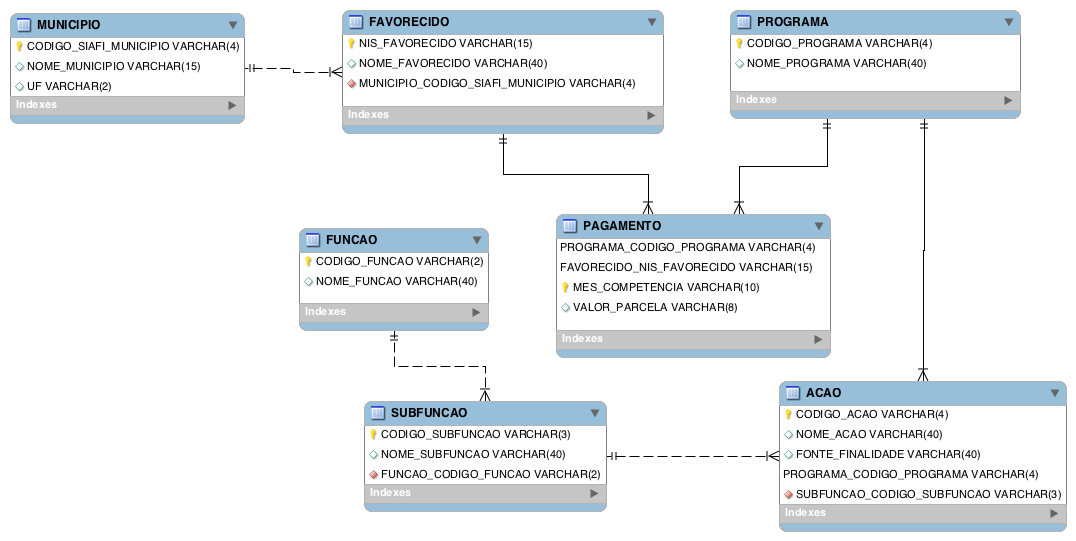
\includegraphics[width=1\textwidth]{eer.png}
		\caption{Modelo relacional do banco de dados dos pagamentos do Programa Bolsa Família (PBF).}
		\label{fig:mr}
	\end{figure}
	
	As entidades, atributos e relações do MR foram descritas na Seção~\ref{sec:der}. 
	
	A partir deste MR o software disponibiliza gerar um \textit{script} de criação das tabelas apresentadas no diagrama, portanto, este foi gerado e utilizado. Na Seção~\ref{sec:etl} iremos explicar melhor como foi realizada a parte de ETL (Extract, Transform, Load) das tabelas normalizadas apresentadas na Figura~\ref{fig:mr}.
	
	\section{Formas Normais}
	\label{sec:fnormais}
	
	Como foi possível observar na Seção~\ref{sec:der} e Seção~\ref{sec:mr} já foram apresentadas soluções normalizadas pois a tabela original que foi obtida através de um arquivo do tipo \textit{CSV} possui 12 atributos na mesma tabela. Na Seção~\ref{sec:etl} será exposto mais informações a respeito da extração, transformação e população das tabelas cruciais ao sistema aqui apresentado.
	
	\subsection{1FN}
	\label{sec:1fn}
	
	A primeira forma normal (1FN) apresenta uma solução onde toda tabela é minimamente normalizada, sendo, o valor de cada coluna indivisível: \\
	
	\begin{center}
		(UF, CODIGO-SIAFI-MUNICIPIO, NOME-MUNICIPIO, CODIGO-FUNCAO, CODIGO-SUBFUNCAO, CODIGO-PROGRAMA, CODIGO-ACAO, NIS-FAVORECIDO, NOME-FAVORECIDO, FONTE-FINALIDADE, VALOR-PARCELA, MES-COMPETENCIA) 
		\label{tab:1fn}
	\end{center} 
	
	Nesta forma os resultados apresentam muita redundância de dados, principalmente ao lidar com um banco de dados extenso como este. Também possui problemas de inserção, remoção e atualização. Logo na próxima sub-seção vamos apresentar uma forma normal mais enxuta. 
	
	\subsection{2FN}
	\label{sec:2fn}
	
	Avaliando às dependências funcionais dos atributos é possível gerar a segunda forma normal (2FN). Se a tabela está em 1FN e todo atributo do complemento de uma chave candidata é \textbf{totalmente funcionalmente dependente} daquela chave então a tabela estará em 2FN:
	
	\begin{center}
		1$ª$ Tabela \\ (CODIGO-SIAFI-MUNICIPIO) $\rightarrow$ NOME-MUNICIPIO, UF \\
		2$ª$ Tabela \\
		(NIS-FAVORECIDO) $\rightarrow$ NOME-FAVORECIDO \\
		3$ª$ Tabela \\
		(CODIGO-PROGRAMA, CODIGO-ACAO) $\rightarrow$ CODIGO-FUNCAO, CODIGO-SUBFUNCAO, FONTE-FINALIDADE \\
		4$ª$ Tabela \\
		(NIS-FAVORECIDO, MES-COMPETENCIA, CODIGO-PROGRAMA) $\rightarrow$ VALOR-PARCELA \\
		\label{tab:2fn}
	\end{center} 
	
	Mesmo na forma 2FN ainda possuem atributos transitivamente dependentes, logo, na próxima sub-seção vamos estudar estes casos para uma maior melhora das tabelas.
	
	\subsection{3FN}
	\label{sec:3fn}
	
	A transitividade de dependência nos permite melhorar as tabelas encontradas da sub-seção anterior, portanto, se uma tabela está na forma 2FN e todos os atributos não-chave forem \textbf{dependentes não-transitivos} de chave primária teremos uma relação de normalização 3FN:
	
	\begin{center}
		1$ª$ Tabela \\ (CODIGO-SIAFI-MUNICIPIO) $\rightarrow$ NOME-MUNICIPIO, UF \\
		2$ª$ Tabela \\
		(NIS-FAVORECIDO) $\rightarrow$ NOME-FAVORECIDO \\
		3$ª$ Tabela \\
		(CODIGO-PROGRAMA, CODIGO-ACAO) $\rightarrow$ CODIGO-SUBFUNCAO, FONTE-FINALIDADE \\
		4$ª$ Tabela \\
		(NIS-FAVORECIDO, MES-COMPETENCIA, CODIGO-PROGRAMA) $\rightarrow$ VALOR-PARCELA \\
		5$ª$ Tabela \\
		(CODIGO-SUBFUNCAO) $\rightarrow$ NOME-SUBFUNCAO \\
		6$ª$ Tabela \\
		(CODIGO-FUNCAO) $\rightarrow$ NOME-FUNCAO 
		\label{tab:3fn} 
	\end{center} 
	
		A 3$ª$ tabela foi alterada pois o CODIGO-FUNCAO é dependente transitivo da chave composta (CODIGO-PROGRAMA, CODIGO-ACAO). A tabela 6 serviu para separar esta dependência transitiva da tabela 3. 
		
		A tabela 5 surgiu somente para fins de clareza do significado do CODIGO-SUBFUNCAO do programa e ação. O atributo de NOME-FUNCAO foi adicionado na tabela 6 pela mesma justificativa.
	
	\section{Extract, Transform, Load (ETL)}
	\label{sec:etl}
	
	A extração, transformação e carregamento dos dados foi realizada de acordo com os seguintes passos:
	
	\begin{enumerate}
		\item Fazer o download dos arquivos CSV disponíveis no \cite{portal};
		\item Extrair os arquivos baixados que vieram em formato ZIP de compreensão na pasta de desenvolvimento do projeto;
		\item Estudar o conteúdo dos arquivos extraídos;
		\item Pré-processar os arquivos extraídos para importar para um formato de banco de dados;
		\item Importar os arquivos CSV pra um arquivo único de DB (Database);
		\item Criar tabelas e popular as tabelas normalizadas utilizando as tabelas originais extraídas.
	\end{enumerate}
	
	As etapas 1 e 2 pertencem à parte de extração dos dados, já as etapas 3, 4 e 5 fazem parte do processo de transformação dos dados. A etapa 6 é elemento do processo de carga de dados.
	
	\subsection{Extract}
	\label{sec:e}
	
	A extração dos dados foi obtida através do \cite{portal}. Foi possível obter dados aberto sobre o Programa Bolsa Família (PBF), utilizando como objeto de estudo um determinado ano e mês. Também foram extraídos dados aberto sobre a Função e Subfunção de recursos e gastos diretos do governo federal.
	
	A primeira extração foi sobre os pagamentos da Bolsa Família para cada favorecido na data de Setembro/2015. A segunda extração foi sobre a Classificação Funcional da Despesa (MTO), onde, possui informações em formato aberto da classificação funcional da Despesa, publicada no Manual Técnico de Orçamento, pelo Ministério do Planejamento, do ano de 2015.
	
	O \cite{portal} disponibiliza arquivos de formato CSV (Comma-separated values) sobre todos os dados lá contidos. Os arquivos CSV foram baixados e extraídos na pasta de desenvolvimento do projeto.
	
	\subsection{Transform}
	\label{sec:t}
	
	Como foi dito na etapa 3, os arquivos foram estudados e analisados antes da importação para um arquivo de banco de dados. Na análise foram descobertos dois problemas:
	
	\textbf{PROBLEMA 1}: Os arquivos não eram de fato do formato CSV e sim TSV (Tab-separated values). 
	
	\textbf{PROBLEMA 2}: Os nomes dos atributos de cada "coluna" possuíam codificação não padrão, ou seja, acento nas palavras. 
	
	Sendo assim, diante destes 2 problemas encontrados foram pesquisadas soluções para tratar os dados extraídos.
	
	\textbf{SOLUÇÃO PARA O PROBLEMA 1}: Utilizar SQLite 3 e Python 3 para tratar as importações dos arquivos TSV para arquivos DB, pois, eles dão suporte para importar este tipo de formato.
	
	\textbf{SOLUÇÃO PARA O PROBLEMA 2}: Implementar um script para substituir a primeira linha do arquivo extraído com nomes válidos para tratar.
	
	Dada as soluções acima elas foram executadas e os resultados foram obtidos com sucesso. Estes problemas foram resolvidos nas etapas 4 e 5 do processo de ETL. 
	
	\subsection{Load}
	\label{sec:l}
	
	Na etapa 6 ficou estipulado que as tabelas obtidas do MR apresentado na Seção~\ref{sec:mr} seriam criadas e populadas a partir das tabelas originais extraídas das fontes externas de dados abertos.
	
	Após a extração e tratamento destes dados foi alcançada a parte de carga de dados nas tabelas normalizadas 3FN. 
	
	\begin{itemize}
		\item Primeiramente o script SQL de criação das tabelas gerado pelo software \cite{mysql} foi modificado para se adequar à linguagem aceita pelo SQLite 3;
		\item Foram estudadas "QUERIES" para extrair os dados das tabelas originais e inserir nas tabelas normalizadas de forma adequada;
		\item Implementação das "QUERIES";
		\item Execução das "QUERIES" utilizando Python 3 e o SQLite 3 (processo bastante demorado).
	\end{itemize}
	
	Entretanto, pela demora de carregamento e processamento dos dados, foi decidido que \textbf{apenas 1000 linhas} das 13 milhões do banco seriam utilizadas, devido a tabela de pagamentos. Desse modo, as perguntas gerais, situadas na seção \ref{sec:resultados} não poderão ser respondidas nesse sistema simplificado.
	
	Por fim, ao final do processo de ETL os dados estão disponíveis para realizar o CRUD (Create, Read, Update e Delete).
	
	\section{Camadas do Sistema para o CRUD}
	\label{sec:camadas}
	
	Com os dados prontos para realizar o CRUD (Create, Read, Update e Delete) chega o momento de implementar um sistema para ler estes dados e apresentar a algum usuário do sistema. O \textit{Design Pattern} de Persistência e Apresentação foi sugerido para aplicação. Como já estava sendo utilizado a linguagem de programação Python 3 no processo de importação dos dados abertos, foi então considerado em dar continuidade à utilização da linguagem para desenvolvimento do sistema.
	
	Por experiências prévias com Web Service com Python 3 e o Framework Web Flask de um membro da equipe que produziu este sistema foi então decidido a utilização destas ferramentas para implementar o sistema que irá executar o CRUD.
	
	\subsection{Persistência}
	\label{sec:pers}
	
	A camada de persistência foi implementada utilizando o SQLite 3 e Python 3 para ler e escrever os dados no arquivo de banco de dados. Tanto a leitura quanto a escrita de algum dado seria passada através de alguma requisição do usuário na camada de Apresentação.
	
	\subsection{Apresentação}
	\label{sec:apt}
	
	Foram utilizadas ferramentas como HTML e CSS para desenhar a camada de apresentação ao usuário. A ponte entre os \textit{templates} HTML e a camada de persistência é feita pelo Framework Web Flask.
	
	\section{Consultas} 
	\label{sec:consultas}
	
	Foram elaborados scripts de consultas para interagir com o banco de dados obtido além do CRUD básico. As consultas elaboradas servem para facilitar a obtenção e leitura de dados do banco de dados. Abordaremos as \emph{queries}, \emph{views} e \emph{triggers} utilizados. Como o SQLite 3 não tem suporte para \emph{procedures}, não foi possível implementá-los neste projeto.
	
	\subsection{Queries}
	\label{sec:query}
	
	As \emph{queries} realizadas tem como objetivo responder às seguintes perguntas:
	
	\begin{itemize}
		\item Quem foi a pessoa que mais recebeu recurso do governo em um determinado ano/mês?
		\item Qual o estado que mais recebeu recurso?
		\item Quem são todos os favorecidos do programa Bolsa Família de Setembro de 2015 organizados em ordem alfabética?
		\item Quantos favorecidos existem por estado?
		\item Qual a média da parcelas?
		\item Qual a média de pagamentos por estado?
	\end{itemize}
	
	\subsection{Views}
	\label{sec:view}
	
	A \emph{view} que utilizamos tem como objetivo mostrar os favorecidos que mais foram beneficiados nesse mês de setembro de 2015. Essa \emph{view} nos mostra o NIS e o nome do favorecido, o total recebido e o mês em que foi recebido, ordenados pelo total recebido por cada pessoa, do mais beneficiado ao menos beneficiado.
	
	\subsection{Procedures}
	\label{sec:proc}
	
	Como dito anteriormente, a biblioteca que usamos, SQLite 3, não tem suporte para \emph{procedures}, portanto não foi possível fazer uso de tal função.
	
	\subsection{Triggers}
	\label{sec:trig}
	
	O \emph{trigger} utilizado tem o fim de gerar um \emph{drop} para cada pagamento de um favorecido que foi removido da tabela. Ou seja, sempre que um favorecido for removido da tabela de favorecidos, todos os pagamentos referentes a esse favorecido também serão removidos. Caso não haja pagamento ao favorecido, nenhum pagamento será removido.
	
	\section{Análise dos Resultados e Considerações Finais}
	\label{sec:resultados}
	
	Foi implementado um sistema capaz de ler e escrever dados abertos de Setembro de 2015 sobre o programa Bolsa Família, com o objetivo responder algumas questões levantadas sobre esta base de dados como:
	
	\begin{itemize}
		\item Quem foi a pessoa que mais recebeu  recurso do governo em um determinado ano/mês?
		\item Qual o estado que mais recebeu recurso?
	\end{itemize}
	
	Também foi descoberto que existe mais de um pagamento direcionado a um mesmo favorecido, do mesmo programa no mesmo mês/ano. Além disso, nesse período de setembro de 2015, foram registradas 13 912 767 entradas de pagamento, deixando o processamento realmente lento. E, para dificultar o processo, para cada FK o SGBD conferia se existia tal chave nas outras tabelas, o que deixou o processo de criação dessa tabela exponencialmente lento.
	
	Portanto, foi decidido que a tabela de pagamentos teria um campo extra chamado \emph{cod{\_}pag}, sendo ele de \emph{auto{\_}increment}. Essa alteração, entretanto, acarretou em mudanças no BD, já que a entidade \emph{Pagamento} deixa de ser entidade fraca, e as relações entre \emph{Favorecido} e \emph{Programa} deixam de ser de identificação.
	
	Por fim, por causa da lentidão no processamento de dados, não foi possível analisar o banco de dados inteiro. Desse modo, foi utilizado \textbf{apenas as primeiras 1000 tuplas} do banco, limitando as tabelas a um máximo de 1000 linhas. Somente assim foi possível de extrair alguns dados do banco e testar as consultas. Por causa dessa redução de dados, não foi possível responder às perguntas gerais citadas acima.
	
	Todo o sistema e scripts de ETL estão no repositório aberto do GitHub criado para o desenvolvimento deste projeto: \url{https://github.com/Dayof/OpenData_BolsaFamilia}. As bases de dados de formato CSV e DB não estão neste repositório remoto devido à extensão destes.
	
\bibliographystyle{sbc}
\bibliography{relatorio} 

%\newpage 
	
\end{document}
